\chapter{Experiments and results}
This section discusses the various experiments pertaining to the proposed hypothesis and their findings. 
\section{Description of Dataset}
The goal of our approach is to establish a system that gives a strong reward-to-risk ratio. A diversified portfolio yields a better return per risk. Our dataset covers daily measurements between the years 2000 and 2022. Every quarter, we retrain our model and update the parameters using all the data we have up to that time. Our testing period spans the years 2000 to the end of June 2022, which includes the most current COVID-19-related crises.
\section{Baseline Algorithms}
We contrast our approach with a collection of standard algorithms. Many pension funds' reallocation techniques make up the first group of baseline models. These strategies allocate important assets according to a predefined allocation ratio, and they rebalance portfolios quarterly to keep these ratios constant. A portfolio may be chosen by investors depending on their preferred level of risk. Generally speaking, portfolios with a higher proportion of stocks would perform better but with more volatility.

Mean-variance optimisation (MV) [20], maximum diversification (MD) [32] and Risk Parity (RP) make up the second group of comparison models. To calculate the anticipated returns and covariance matrix, we employ moving averages with a 50-day rolling window. We choose weights for the portfolio that maximise the Sharpe ratio for MV on a daily basis. The diversity-weighted portfolio (DWP) from stochastic portfolio theory, as reported in [28], , links portfolio weights to asset market capitalisation, it is possible to consistently outperform the market index [10]. The final baseline method, known as Risk Parity Portfolio (RP), creates optimal portfolios by optimising the basic risk parity model \cite{Bruder2012}.
\subsection{Training Scheme}
In this study, we model the portfolio weights using a single layer of 64-unit LSTM connectivity in order to optimise the Sharpe ratio. Instead of carefully adjusting the "appropriate" hyperparameters, we purposefully make our network simple to demonstrate the efficiency of our end-to-end training process. Each market index's closing prices and daily returns are included in our input, which is made up of observations over the previous 50 days. Keeping returns helps with the analysis of (Eq 7) and we can also use them as momentum characteristics in [26]. We are aware that returns may indeed be calculated from prices. We chose these frequently utilised features for our work since choosing features is not our main emphasis. Our network is trained using the Adam optimiser [17], and the mini-batch size is 64. For the purpose of optimising hyperparameters and preventing overfitting issues, we segregate 10\% of every training data into a separate validation set. The validation set is used for any hyperparameter optimisation, leaving the test data for the final performance assessment and confirming the reliability of our findings. Our training method typically ends after 100 epochs.

\section{Experiments}
\graphicspath{ {images/} }
\subsection{Correlation Heatmap}
\begin{figure}[H]
\centering
   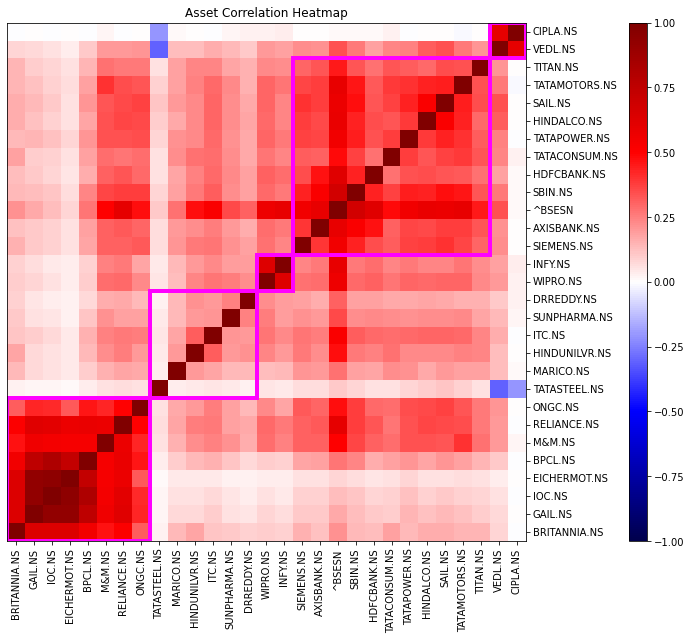
\includegraphics[width=1.0\textwidth]{correlation.png}
      \caption{Correlation Heatmap}
       \label{corel}
\end{figure}

\subsection{Experiments Parameters}
\subsubsection{Optimisation}
Start date = 2000-01-01\\
End Date = 2022-07-31\\
Risk Free Rate = 0 (For Simplicity)
\subsubsection{BackTesting}
Start Money = 10,00,000\\
Commission = 0.5\%\\
Silppage = 0.5\%\\
Benchmark Index = BSE Sensex\\

\subsection{Benchmark Experiment}
\subsubsection{Experiment Description}
It's crucial to have a precise and clear method to measure your portfolio since a financial market's aspects are always changing. In order to do this, benchmark portfolios should provide investors with a realistic assessment of how their portfolio are performing relative to the important and specialised market categories.\\\\
We can evaluating our portfolio's total performance with respect to predetermined benchmarks, such as a market indices or a group of asset classes, by using a benchmark portfolio. These indexes are "passive" and unmanaged, in contrast to the actively managed investment portfolio that makes up your overall investment portfolio. As a result, benchmark portfolios may be used to assess the value a manager brings to your portfolio.\\\\
We are going to use BSE Sensex as Benchmark Portfolio\\\\
\textbf{Theory}
The benchmark index of BSE is referred as Sensex.  The 30 biggest and most popular companies on the BSE make up the Sensex, which serves as a bellwether for the Indian economy. It is market capitalisation-weighted and float-adjusted. Every year, between June and December, the Sensex is evaluated and Rebalanced. The Sensex is run by Standard \& Poor's and is the earliest known stock index in India, having been founded in 1986. It is used by analysts and investors to track the economic cycles in India as well as the growth and decline of certain sectors.
\subsubsection{Results}
\begin{figure}[H]
\centering
   \includegraphics[width=1.0\textwidth]{Benchmark/allocation.png}
      \caption{Allocation of assets of Sensex}
       \label{benchmark_alloc}
\end{figure}
\begin{figure}[H]
\centering
   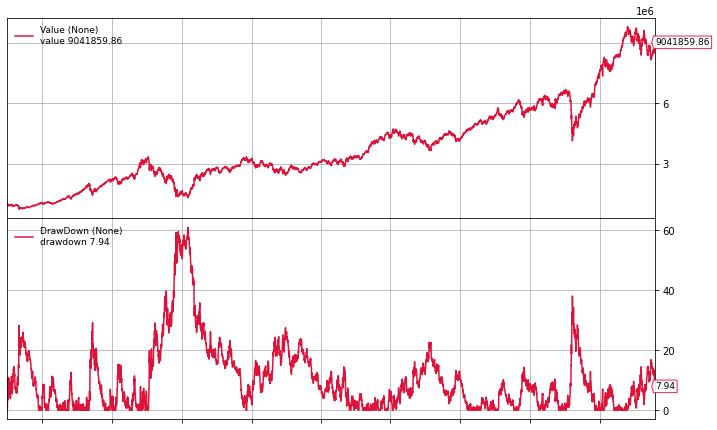
\includegraphics[width=1.0\textwidth]{Benchmark/backtest.png}
      \caption{Backtest and Drawdown of Benchmark}
       \label{benchmark}
\end{figure}


\begin{table}[H]
\centering
\begin{tabular}{|c | c|} 
 \hline
 Max Drawdown: &60.88\%\\
CAGR: &10.54\%\\
Sharpe: &0.514\\
Final Portfolio Value: &9041859.86\\
 \hline
\end{tabular}
\caption{Outcomes of the Benchmark Experiment}
\label{becnhmark outcome table}
\end{table}
\subsubsection{Conclusion}
Since the inception of BSE Sensex in 2000 (base year), we have seen the worst downfall in 2008 of 60.88\% and a significant decline in 2020. Sensex has given a CAGR of 10.54\% since its inception, with a Sharpe ratio of 0.514. A lump sum investment of Rs 10 Lack in Sensex in 2000 would be Rs 90 Lack 41 thousand in Present Date 
\subsection{Mean Variance Optimisation}
\subsubsection{Experiment Description}
The objective of creating a portfolio of assets using modern portfolio theory (MPT), also known as mean-variance optimisation, is to maximise anticipated return for a certain degree of risk. It formalises and broadens the concept of diversity in investment, which holds that having a variety of financial assets reduces risk compared to holding a single kind. Its main conclusion is that an investment's return and risk should not be evaluated on its own, but rather in the context of the risk and return of the whole portfolio. It substitutes asset price variation for risk.\\
\textbf{Theory}
\[\underset{w}{\max}\qquad \frac{R (w) - r_{f}}{\phi(w)}\]
Where:

$R(w)$ is the return function:

$w$: is the vector of weights of the portfolio.

$\phi(w)$: Standard Deviation of the portfolio.

$r_{f}$: is the risk free rate.\\
\subsubsection{Results}

\begin{figure}[H]
\centering
   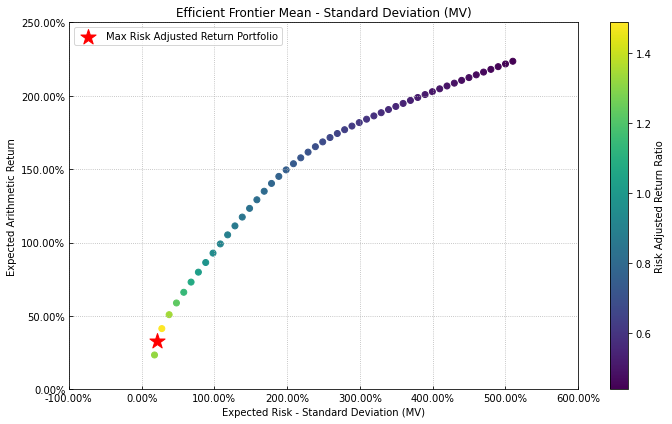
\includegraphics[width=1.0\textwidth]{MV/EF.png}
      \caption{Efficient Frontier of Mean Variance Portfolio}
       \label{MV_EF}
\end{figure}
\begin{figure}[H]
\centering
   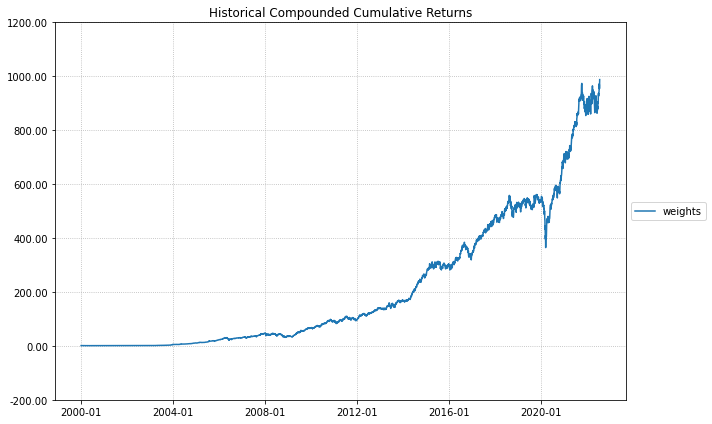
\includegraphics[width=1.0\textwidth]{MV/Historic.png}
      \caption{Historic Compounded Cumulative Returns using Mean Variance}
       \label{MV_HCCR}
\end{figure}

\begin{figure}[H]
\centering
   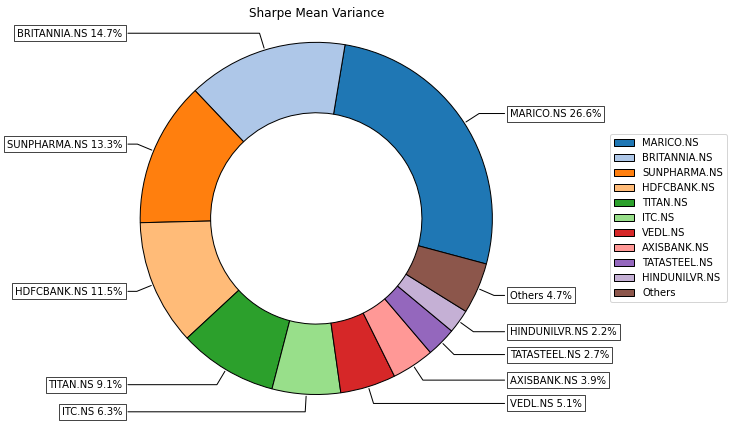
\includegraphics[width=1.0\textwidth]{MV/Allocation.png}
      \caption{Allocation of assets using Mean Variance}
       \label{MV_Alloc}
\end{figure}

\begin{figure}[H]
\centering
   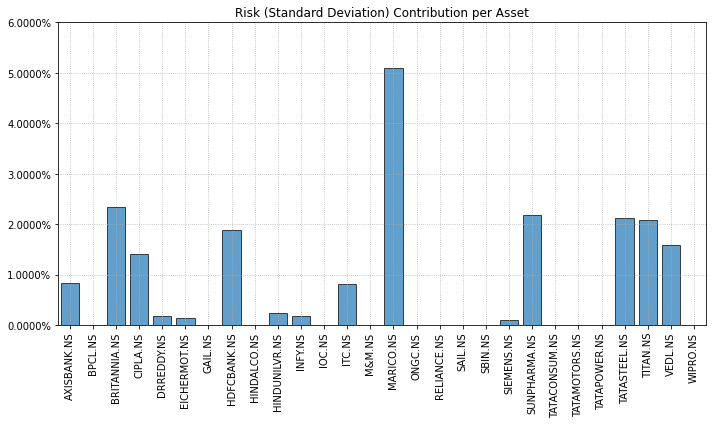
\includegraphics[width=1.0\textwidth]{MV/Risk.png}
      \caption{Risk Contribution Per Asset}
       \label{MV_Risk}
\end{figure}

\subsubsection{Backtest and Drawdown of Mean Variance Oprimisation}

\begin{figure}[H]
\centering
   \includegraphics[width=1.0\textwidth]{MV/Backtest.png}
      \caption{Backtest and Drawdown of Mean-Variance Optimisation}
       \label{MV_backtest}
\end{figure}

\begin{table}[H]
\centering
\begin{tabular}{|c | c|} 
 \hline
 Max Drawdown: &41.59\%\\
CAGR: &17.00\%\\
Sharpe: &0.780\\
Final Portfolio Value: &31998532.49\\
 \hline
\end{tabular}
\caption{Outcomes of the Mean Variance Experiment}
\label{MV outcome table}
\end{table}
\subsubsection{Conclusion}
Since the Start of our study in 2000 (base year), We have seen the worst downfall in 2008 of 41.59\% and a significant decline in 2020. Mean Variance optimisation has given a CAGR of 17.00\% since its inception, with a Sharpe ratio of 0.780. A lump sum investment of Rs 10 Lack in portfolio using Mean Variance optimisation in 2000 would be Rs 3 Crore 19 Lack and 98 thousand in Present Date
\subsection{Maximum Diversification Optimisation}
\subsubsection{Experiment Description}

One of the most crucial factors to take into account when building an investing portfolio is spreading assets out to lower risk. One strategy is to diversify as much as possible. It is a portfolio strategy that seeks to build the most diversified portfolio achievable. The strategy specifically aims to increase the diversification ratio. Hence, the greatest diversity method is a risk-based allocation strategy than ignores predicted returns. The strategy aims to create a portfolio with a wide range of investments.\\\\
\textbf{Theory}\\

\[\underset{w}{\min}\qquad \frac{P' (w) \cdot \Sigma}{\sqrt{P'VP}}\]
Where:

$P$: is the portfolio weights.

$\Sigma$: is the asset volatilities.

$V$: covariance matrix of these assets.

$r_{f}$: is the risk free rate.\\

\subsubsection{Results}

\begin{figure}[H]
\centering
   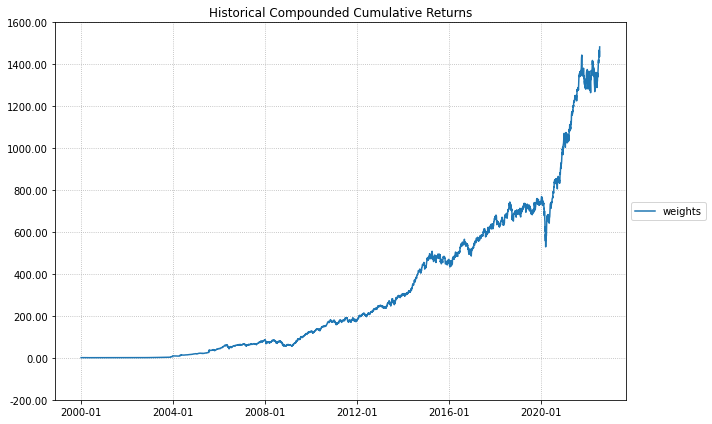
\includegraphics[width=1.0\textwidth]{MD/Historic.png}
      \caption{Historic Compounded Cumulative Returns Using Maximum Diversification}
       \label{MD_HCCR}
\end{figure}

\begin{figure}[H]
\centering
   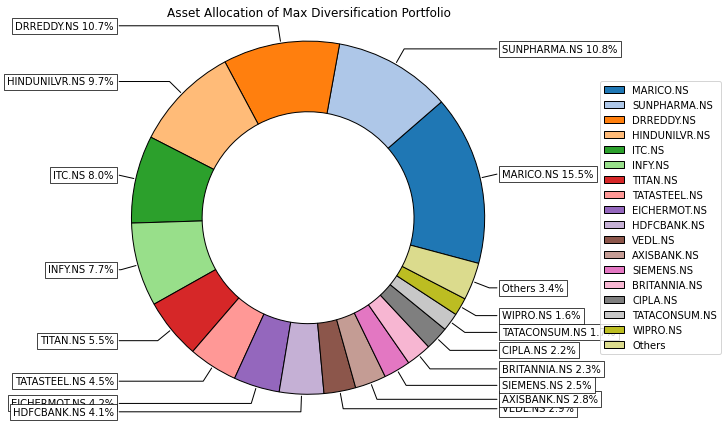
\includegraphics[width=1.0\textwidth]{MD/Allocation.png}
      \caption{Allocation of assets using Maximum Diversification}
       \label{MD_Alloc}
\end{figure}

\begin{figure}[H]
\centering
   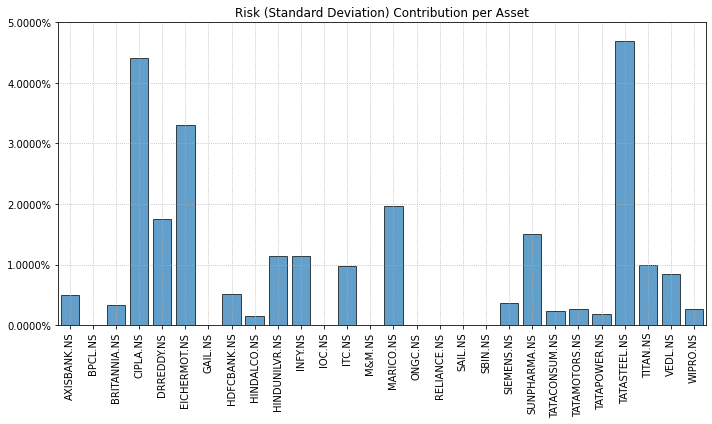
\includegraphics[width=1.0\textwidth]{MD/Risk.png}
      \caption{Risk Contribution Per Asset}
       \label{MD_Risk}
\end{figure}

\subsubsection{Back Testing With Maximum Diversification Strategy on Assets}

\begin{figure}[H]
\centering
   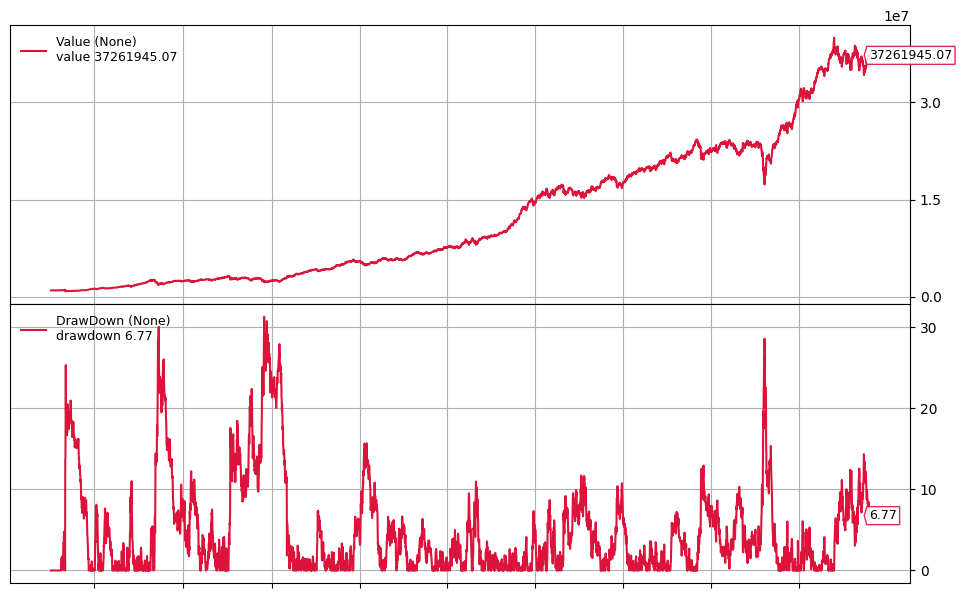
\includegraphics[width=1.0\textwidth]{MD/backtest.png}
      \caption{Backtest and Drawdown of Maximum Diversification Optimisation
}
       \label{MD_assets}
\end{figure}

\begin{table}[H]
\centering
\begin{tabular}{|c | c|} 
 \hline
 Max Drawdown: &31.31\%\\
CAGR: &17.85\%\\
Sharpe: &0.911\\
Final Portfolio Value: &37261945.07\\
 \hline
\end{tabular}
\caption{Outcomes of the Maximum Diversification Experiment}
\label{MD outcome table}
\end{table}
\subsubsection{Conclusion}
Since the Start of our study in 2000 (base year), We have seen the worst downfall in 2008 of 31.31\% and a significant decline in 2020. Maximum Diversification optimisation has given a CAGR of 17.85\% since its inception, with a Sharpe ratio of 0.911. A lump sum investment of Rs 10 Lack in portfolio using Mean Variance optimisation in 2000 would be Rs 3 Crore 72 Lack and 61 thousand in Present Date

\subsection{Risk Parity Portfolio Optimisation}
\subsubsection{Experiment Description}
An method to asset management known as risk parity optimisation places more emphasis on risk allocation rather than capital allocation, which is often referred to as volatility. According to the risk parity method, the risk parity portfolio may produce a better Sharpe ratio and can be more resilient to market downturns than the standard portfolio when asset allocations are modified to the same risk level. Risk parity is susceptible to substantial changes in correlation regimes, as was seen in Q1 2020, which caused risk-parity funds to perform much worse than average during the Covid-19 sell-off.

\textbf{Theory}

\[\begin{aligned}
&\underset{w}{\min} & & \phi(w) \\
&\text{s.t.} & & b \log(w) \geq c \\
& & & w \geq 0 \\
\end{aligned}\]
Where:

$w$: weights of the portfolio.

$b$: risk contribution constraints.

$\phi(w)$: Standard Deviation of the portfolio

$c$: is an arbitrary constant.

\subsubsection{Results}

\begin{figure}[H]
\centering
   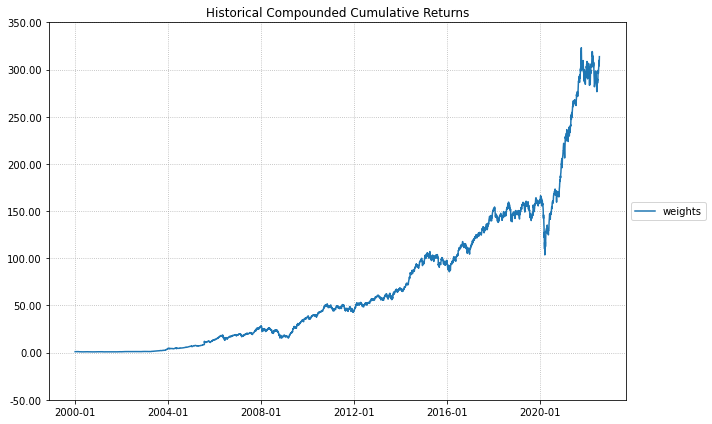
\includegraphics[width=1.0\textwidth]{RP/Historic.png}
      \caption{Historic Compounded Cumulative Returns Using Risk Parity}
       \label{RP_HCCR}
\end{figure}

\begin{figure}[H]
\centering
   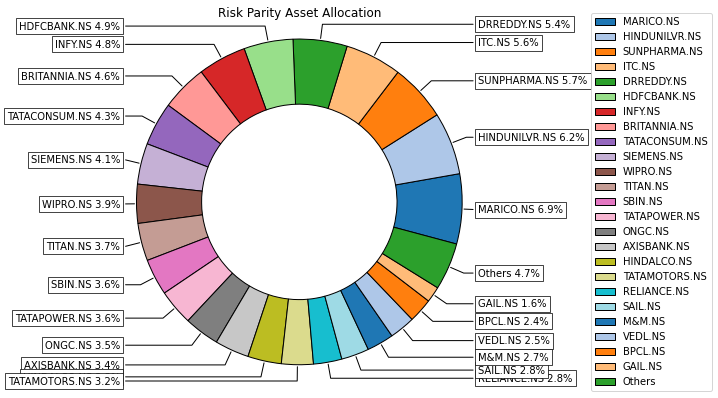
\includegraphics[width=1.0\textwidth]{RP/Allocation.png}
      \caption{Allocation of assets using Risk Parity}
       \label{RP_Alloc}
\end{figure}

\begin{figure}[H]
\centering
   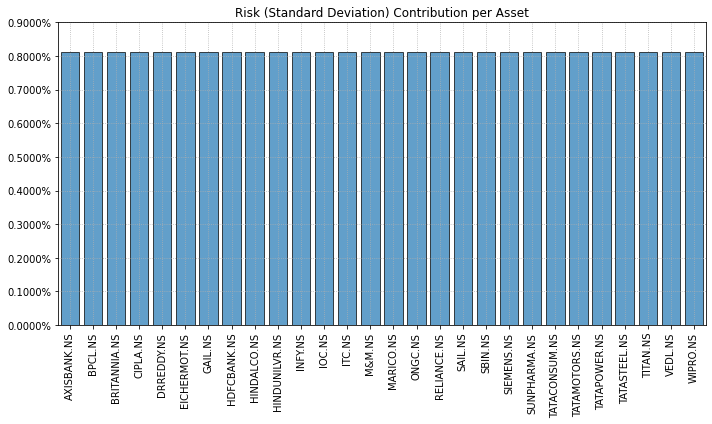
\includegraphics[width=1.0\textwidth]{RP/Risk.png}
      \caption{Risk Contribution Per Asset}
       \label{RP_Risk}
\end{figure}

\subsubsection{Back Testing With Risk Parity Strategy on Assets}

\begin{figure}[H]
\centering
   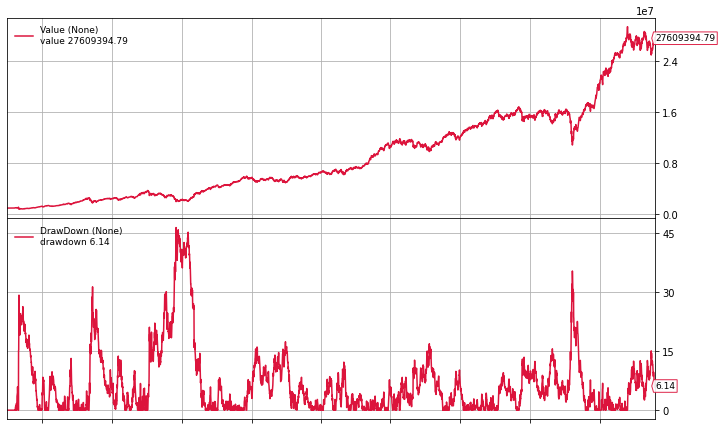
\includegraphics[width=1.0\textwidth]{RP/backtest.png}
      \caption{Backtest and Drawdown of Risk Parity Optimisation
}
       \label{fig:RP_assets}
\end{figure}

\begin{table}[H]
\centering
\begin{tabular}{|c | c|} 
 \hline
 Max Drawdown: &46.45\%\\
CAGR: &16.27\%\\
Sharpe: &0.697\\
Final Portfolio Value: &27609394.79\\

 \hline
\end{tabular}
\caption{Outcomes of the Risk Parity Experiment}
\label{RP outcome table}
\end{table}
\subsubsection{Conclusion}
Since the Start of our study in 2000 (base year), We have seen the worst downfall in 2008 of 46.45\% and a significant decline in 2020. Risk Parity optimisation has given a CAGR of 16.27\% since its inception, with a Sharpe ratio of 0.697. A lump sum investment of Rs 10 Lack in portfolio using Mean Variance optimisation in 2000 would be Rs 2 Crore 76 Lack and 9 thousand in Present Date

\subsection{LSTM based Portfolio Optimisation}
\subsubsection{Experiment Description}
This study considers using deep learning models to directly optimise a portfolio.  We avoid this forecasting phase in favour of getting asset allocations immediately, in contrast to traditional techniques where anticipated returns are first forecasted (usually by econometric models). Since the prediction stages aim to minimise a prediction loss that is not the total reward from the portfolio, the return forecasting technique is not guaranteed to maximise the performance of a portfolio, as shown by many studies. In contrast, our strategy maximises return per unit of risk by explicitly optimising the Sharpe ratio. In order to maximise the Sharpe ratio, our approach first joins several characteristics from various assets to create a single observation. A neural network is then used to extract the most important information and output portfolio weights.

\textbf{Theory}
\begin{center}
\textit{As Discussed in section \ref{objective function} }
\end{center}
Figure \ref{LSTM_output} displays the model's schematic design. The asset's daily closing prices for the previous 125 days are used as the model's input. The 125-day input data contains two features: close values and percentage change, and it has a form of shape $(125, 2)$. The input layer accepts the data and sends it on to the 64-node initial LSTM layer. The shape produced by the LSTM layer is $(125, 64)$. This indicates that each LSM layer node extracts 64 characteristics from each row throughout the input information. The middle layer is Flatten layer, which converts an n-dimensional array into a 1-dimensional array. The output of the dense layer, which consists of 28 nodes, provides the Asset Allocation's anticipated value. The output layer employs the softmax activation function, commonly referred to as softargmax or the normalised exponential function. An Early Stopping callback Function is implemented  that enables us to give an any large number of learning epochs and discontinue learning whenever the observed parameter stops enhancing
\begin{figure}[H]
\centering
   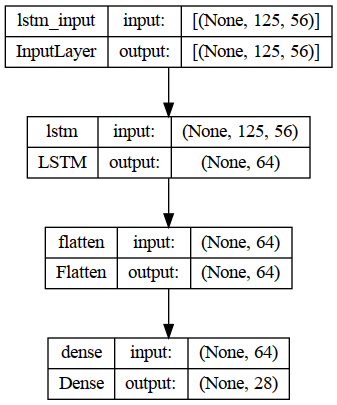
\includegraphics[width=0.5\textwidth]{LSTM/output.png}
      \caption{LSTM model's Schematic diagram}
       \label{LSTM_output}
\end{figure}
\subsubsection{Results}

\begin{figure}[H]
\centering
   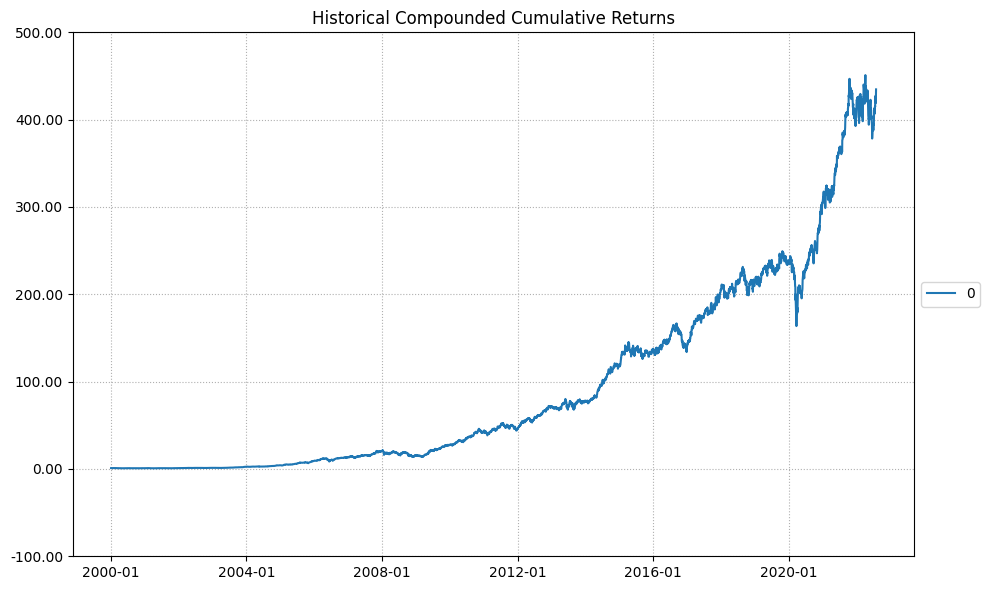
\includegraphics[width=1.0\textwidth]{LSTM/Historic.png}
      \caption{Historic Compounded Cumulative Returns Using LSTM}
       \label{LSTM_HCCR}
\end{figure}

\begin{figure}[H]
\centering
   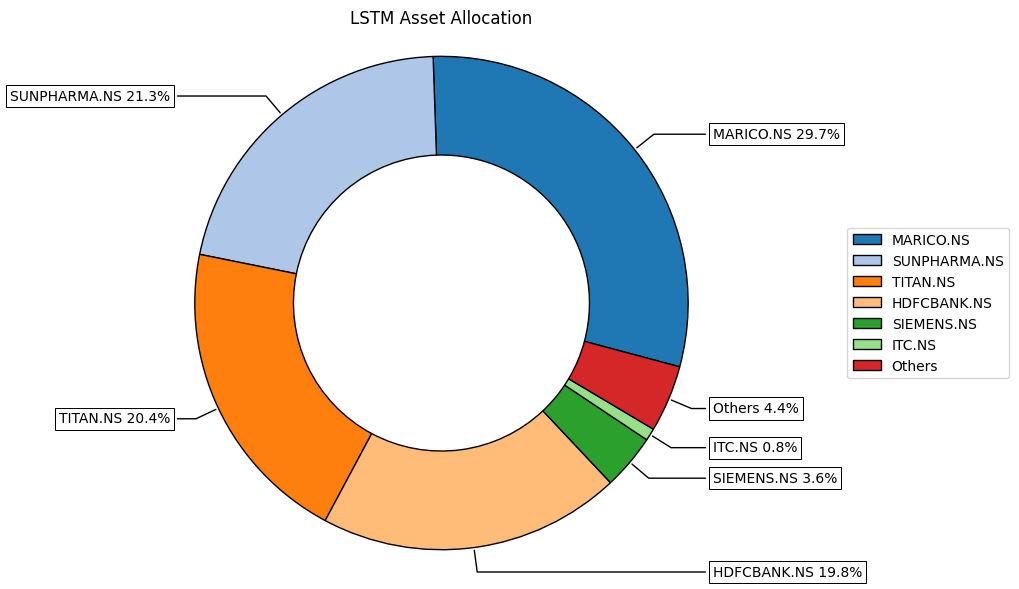
\includegraphics[width=1.0\textwidth]{LSTM/Allocation.png}
      \caption{Allocation of assets using LSTM}
       \label{LSTM_Alloc}
\end{figure}

\begin{figure}[H]
\centering
   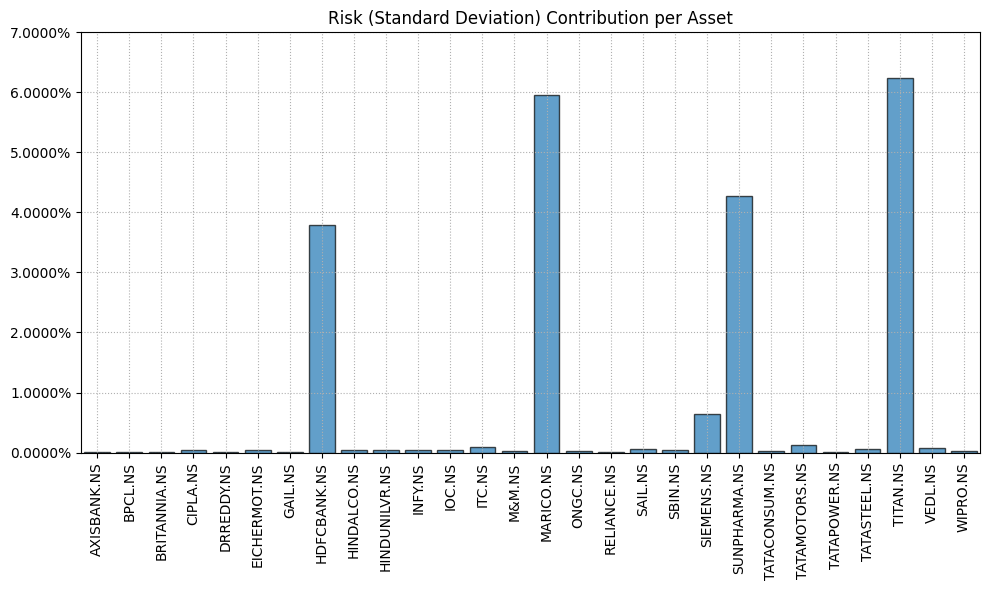
\includegraphics[width=1.0\textwidth]{LSTM/Risk.png}
      \caption{Risk Contribution Per Asset}
       \label{LSTM_Risk}
\end{figure}

\subsubsection{Back Testing With LSTM Strategy on Assets}

\begin{figure}[H]
\centering
   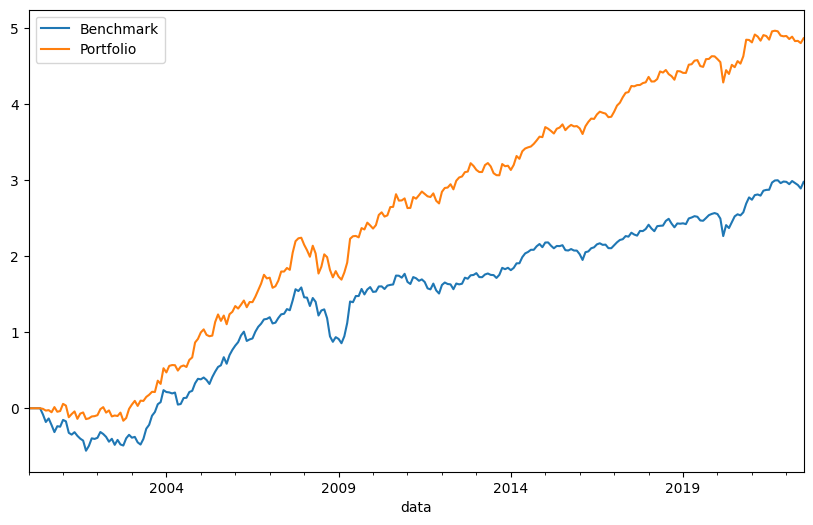
\includegraphics[width=1.0\textwidth]{LSTM/backtest.png}
      \caption{Backtest of LSTM Optimisation
}
       \label{LSTM_assets}
\end{figure}

\begin{table}[H]
\centering
\begin{tabular}{|c | c|} 
 \hline
 Max Drawdown: &55.34\%\\
CAGR: &20.07\%\\
Sharpe: &0.966\\
Final Portfolio Value: &60135137.08\\
 \hline
\end{tabular}
\caption{Outcomes of the LSTM Experiment}
\label{LSTM outcome table}
\end{table}
\subsubsection{Conclusion}
Since the Start of our study in 2000 (base year), We have seen the worst downfall in 2008 of 55.34\% and a significant decline in 2020. LSTM optimisation has given a CAGR of 20.07\% since its inception, with a Sharpe ratio of 0.966. A lump sum investment of Rs 10 Lack in portfolio using Mean Variance optimisation in 2000 would be Rs 6 Crore 1 Lack and 35 thousand in Present Date
\section{Results and Conclusion}
\begin{table}[H]
\centering
\begin{tabular}{|l|l|l|l|l|l|}
\hline
 & Benchmark & MV & MD & RP & LSTM \\ \hline
Max Drawdown: & 60.88\% & 41.59\% & 31.31\% & 46.45\% & 55.34\% \\ \hline
CAGR: & 10.54\% & 17.00\% & 17.85\% & 16.27\% & 20.07\% \\ \hline
Sharpe: & 0.514 & 0.780 & 0.911 & 0.697 & 0.966 \\ \hline
Final Portfolio Value: & 90.41 Lack & 3.2 Crore & 3.73 Crore & 2.76 Crore & 6.01 Crore \\ \hline
\end{tabular}
\caption{Comparison of Outcomes of different Experiments}
\label{tab:Overall Conclusion}
\end{table}
As in Table \ref{tab:Overall Conclusion}, We can conclude that Our LSTM model has outperformed all other optimisation methods with a CAGR of 20.07\% while maintaining a Highest Sharpe ratio of 0.966. Meanwhile, the Sharpe ratio is of Maximum Diversification Optimisation with a value of 0.911 and above average return of 17.85\%. The industry Standard Mean-Variance Optimisation technique has given a return of 17\% with a Sharpe ratio of 0.780. Other than that, Risk parity optimisation has shown 16.27\% CAGR and a reasonable Sharpe ratio of 0.697.
The Benchmark has performed inferior to our experiments with a return of 10.54\% CAGR and a Sharpe Ratio of 0.514
